\chapter{Integers and Floating Point Numbers}

\section{What is Integer?}
An integer (from the Latin integer meaning "whole") [note 1] is a number that can be written without a fractional component. For example, 21, 4, 0, and −2048 are integers, while 9.75, 5½, and √2 are not.

\begin{figure}[h!]
\centering
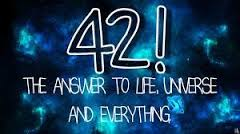
\includegraphics[scale=1.7]{universe.jpg}
\caption{The ultimate answer of the universe is also an Integer!}
\citep{adams1995hitchhiker}
\label{fig:univerise}
\end{figure}

\section{Floating point!}
Also called floats, they represent real numbers and are written with a decimal point dividing the integer and fractional parts. 
You can convert an integer to a floating number by your python and vice versa! :

\begin{verbatim}
Type int(x) to convert x to a plain integer.
                                                                                                            
Type: int(4.22222)
Result: 4


Type float(x) to convert x to a floating-point number.

type: float(1)
Result: 1.0
\end{verbatim}



\section{Number Type Conversion}
Python converts numbers internally in an expression containing mixed types to a common type for evaluation. But sometimes, you need to coerce a number explicitly from one type to another to satisfy the requirements of an operator or function parameter.


